\chapter{AHTR Plank Optimization Results}
In this chapter, I report the \gls{AHTR} plank \gls{ROLLO} optimization results. 
In the previous chapter, I detailed the \gls{AHTR} plank's modeling and \gls{ROLLO} 
optimization methodology. 
Specifically, I described the \gls{AHTR} plank geometry in Section 
\ref{sec:ahtr-plank-geometry}.
I described how I will vary the following \gls{AHTR} plank's input parameters in Section
\ref{sec:input-parameter-modeling}:  
\begin{itemize}
    \item \gls{TRISO} particle packing fraction distribution, 
    $\rho_{TRISO}(\vec{r})$
    \item Total fuel packing fraction
    \item \gls{FLiBe} coolant channel shape 
\end{itemize} 
I described and verified the \gls{AHTR} plank's OpenMC neutronics and Moltres 
temperature models in Sections \ref{sec:ahtr-moltres-hom} and 
\ref{sec:ahtr_model_verification}. 
I described the optimization objectives and how I calculated them from the OpenMC 
and Moltres model outputs in Sections \ref{sec:opt-problem} and 
\ref{sec:ahtr_slab_output}.

In the subsequent sections, I outline single-objective and multi-objective 
ROLLO optimization simulations that are run, and their respective results. 

\section{ROLLO Optimization Simulations Overview}
Table \ref{tab:slab-obj-breakdown} shows the details of each \gls{ROLLO} 
optimization problems explored in this chapter.
\begin{table}[]
    \centering
    \onehalfspacing
    \caption{\acrfull{ROLLO} simulations for optimizing \acrfull{AHTR}
    plank. $PF$: Total Fuel Packing Fraction, $T_{max}$: Maximum Plank Temperature, 
    $PPF$: Normalized Power Peaking Factor, $\rho_{TRISO}(\vec{r})$: 
    \gls{TRISO} particle distribution}
	\label{tab:slab-obj-breakdown}
    \footnotesize
    \begin{tabular}{p{1.4cm}|p{1cm}|llll}
    \hline 
    \textbf{Num of Objs} & \textbf{Sim} & \textbf{Objectives} & \textbf{Constraints} &\textbf{Varying Parameters} & \textbf{Simulation Software} \\
    \hline
    \multirow{9}{2cm}{1}& p-1a & \tabitem max($k_{eff}$) & - &\tabitem $\rho_{TRISO}(\vec{r})$ & OpenMC\\
    \cline{2-6}
    & p-1b & \tabitem min($PF$) & \tabitem $k_{eff}$ $>$ 1.39 &\tabitem $\rho_{TRISO}(\vec{r})$ & OpenMC \\
    & & & & \tabitem $PF$ & \\
    \cline{2-6}
    & p-1c & \tabitem min($T_{max}$) & \tabitem $k_{eff}$ $>$ 1.0 &\tabitem $\rho_{TRISO}(\vec{r})$ & OpenMC, Moltres\\
    \cline{2-6}
    & p-1d & \tabitem min($PPF$) & \tabitem $k_{eff}$ $>$ 1.0 &\tabitem $\rho_{TRISO}(\vec{r})$ & OpenMC\\
    \cline{2-6}
    & p-1e & \tabitem min($PF$) & \tabitem $k_{eff}$ $>$ 1.39 &\tabitem FLiBe channel shape & OpenMC \\
    & & & & \tabitem $PF$ & \\
    \cline{2-6}
    & p-1f & \tabitem min($T_{max}$) & \tabitem $k_{eff}$ $>$ 1.0 &\tabitem FLiBe channel shape & OpenMC, Moltres\\
    \cline{2-6}
    & p-1g & \tabitem min($PPF$) & \tabitem $k_{eff}$ $>$ 1.0 &\tabitem FLiBe channel shape & OpenMC\\
    \hline
    \multirow{6}{2cm}{2}& p-2a & \tabitem min($PF$) & \tabitem $k_{eff}$ $>$ 1.39 & \tabitem $\rho_{TRISO}(\vec{r})$ & OpenMC, Moltres\\
    & &\tabitem min($T_{max}$) & & \tabitem $PF$ & \\
    \cline{2-6}
    & p-2b & \tabitem min($PF$) & \tabitem $k_{eff}$ $>$ 1.39 & \tabitem $\rho_{TRISO}(\vec{r})$ & OpenMC\\
    & & \tabitem min($PPF$) & & \tabitem $PF$ & \\
    \cline{2-6}
    & p-2c & \tabitem min($T_{max}$) & \tabitem $k_{eff}$ $>$ 1.0 & \tabitem $\rho_{TRISO}(\vec{r})$ & OpenMC, Moltres\\
    & & \tabitem min($PPF$) & & & \\
    \hline
    \multirow{3}{2cm}{3}& p-3a &\tabitem min($PF$) & \tabitem $k_{eff}$ $>$ 1.39 & \tabitem $\rho_{TRISO}(\vec{r})$ & OpenMC, Moltres\\
    && \tabitem min($PPF$) & & \tabitem $PF$ & \\
    && \tabitem min($T_{max}$) & & & \\
    \hline
    \end{tabular}
\end{table}
I first conducted single objective, single input parameter \gls{ROLLO} optimizations to 
understand the individual impacts of each objective on each input parameter. 
Their results will inform the multi-objective optimization simulations setup. 

The $k_{eff}$ constraint value is 1.39 and 1.0 for optimization problems that do
and do not minimize total packing fraction, respectively. 
$k_{eff}$ is strongly correlated with total packing fraction. 
The FHR Benchmark's assembly model had a $k_{eff}$ of 1.39, thus, I constrainined
$k_{eff} > 1.39$ to find optimal input parameters that achieve similar performance 
to the original benchmark TRISO distribution. 

\section{AHTR Plank: Single-Objective Optimization Results}

\subsection{Objective: Maximize $k_{eff}$}

\subsubsection{Simulation 1a: Variation of $\rho_{TRISO}(\vec{r})$}

\subsection{Objective: Minimize Total Packing Fraction}
\subsubsection{Simulation 1b: Variation of $\rho_{TRISO}(\vec{r})$ and PF}
Table \ref{tab:simulation1b} shows simulation 1b's optimization problem parameters. 
\begin{table}[H]
    \centering
    \onehalfspacing
    \caption{Simulation 1b Optimization Problem Parameters}
	\label{tab:simulation1b}
    \footnotesize
    \begin{tabular}{l|p{3cm}}
    \hline 
    \multicolumn{2}{c}{\textbf{Single Objective: Simulation 1b}} \\
    \hline 
    \textbf{Objectives} & Minimize PF \\
    \hline 
    \textbf{Input Parameter variations} & $0.02<PF<0.04$ \\
    & $0<a<2$ \\
    & $0<b<\frac{\pi}{2}$ \\
    & $0<c<2\pi$ \\
    \hline
    \textbf{Constraints} & $k_{eff} > 1.39$\\ 
    \hline 
    \textbf{Genetic Algorithm Parameters} & Population size: 60 \\
    & Generations: 10 \\
    \hline
    \end{tabular}
\end{table}
Figure \ref{fig:slab-obj-1-pf-evol} shows the total packing fraction evolution and 
figure \ref{fig:slab-obj-1-pf-final} shows the five TRISO particle distributions in 
the final generation with the most minimized packing fractions. 
\begin{figure}[]
    \centering
    \begin{subfigure}{\textwidth}
        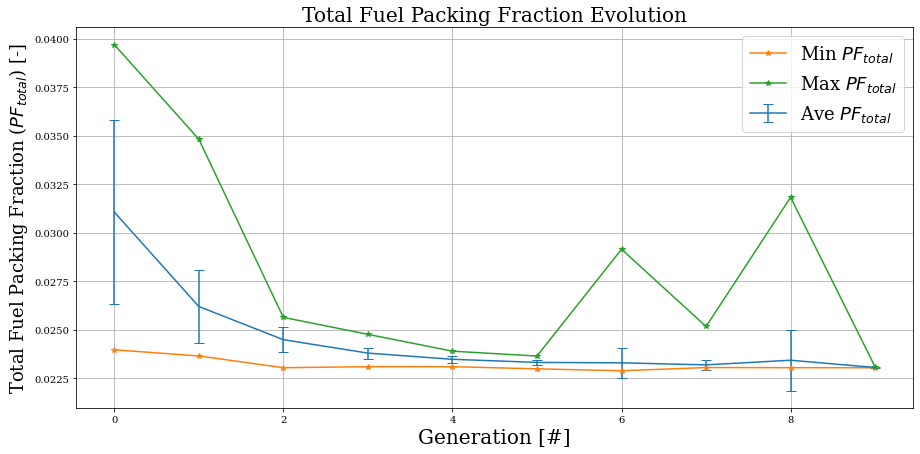
\includegraphics[width=\linewidth]{slab-obj-1-pf-evol.png}
        \caption{Minimum, average, and maximum total packing fraction evolution.}
        \label{fig:slab-obj-1-pf-evol} 
    \end{subfigure}
    \begin{subfigure}{\textwidth}
        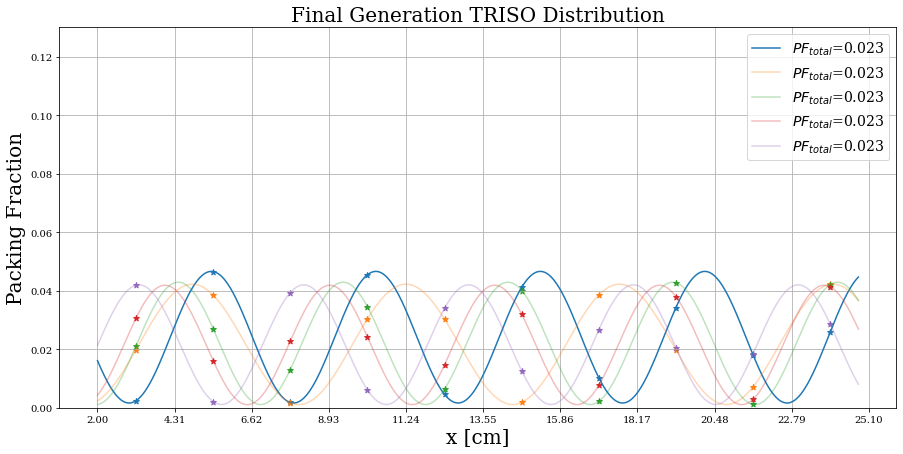
\includegraphics[width=\linewidth]{slab-obj-1-pf-final.png}
        \caption{TRISO particle distribution for the 5 individuals with the 
        smallest packing fraction in generation 9.}
        \label{fig:slab-obj-1-pf-final} 
    \end{subfigure}
    \caption{ROLLO single-objective optimization to minimize total packing fraction. 
    Input parameters varied: total packing fraction, TRISO particle distribution.}
    \label{fig:slab-obj-1-pf}
\end{figure}
The minimum and average packing fractions converged very quickly, as expected 
in this single-objective optimization problem.
By the $9^{th}$ generation, the average, minimum, and maximum packing fraction
values converged to approximately 0.023. 
In figure \ref{fig:slab-obj-1-pf-final}, the TRISO particle packing 
sine distributions are not exactly the same, but follow a similar pattern of 
alternating between a higher packing fraction, and a lower packing fraction 
in the neighboring fuel cell. 
The up-down fuel packing pattern minimizes self-shielding effects, enabling  
a lower packing fraction for the same $k_{eff}$. 

\subsubsection{Simulation 1e: Variation of FliBe Channel Shape and PF}

\subsection{Objective: Minimize Maximum Temperature}

\subsubsection{Simulation 1c: Variation of $\rho_{TRISO}(\vec{r})$}
Table \ref{tab:simulation1c} shows simulation 1c's optimization problem parameters. 
\begin{table}[H]
    \centering
    \onehalfspacing
    \caption{Simulation 1c Optimization Problem Parameters}
	\label{tab:simulation1c}
    \footnotesize
    \begin{tabular}{l|p{3cm}}
    \hline 
    \multicolumn{2}{c}{\textbf{Single Objective: Simulation 1c}} \\
    \hline 
    \textbf{Objectives} & Minimize $T_{max}$ \\
    \hline 
    \textbf{Input Parameter variations} & $0<a<2$ \\
    & $0<b<\frac{\pi}{2}$ \\
    & $0<c<2\pi$ \\
    \hline
    \textbf{Constraints} & $k_{eff} > 1.0$\\ 
    \hline 
    \textbf{Genetic Algorithm Parameters} & Population size: 60 \\
    & Generations: 10 \\
    \hline
    \end{tabular}
\end{table}
Figure \ref{fig:slab-obj-1-temp-evol} shows the plank's $T_{max}$ evolution 
and Figure \ref{fig:slab-obj-1-temp-final} shows the five TRISO particle 
distributions in the final generation with the most minimized $T_{max}$.
\begin{figure}[]
    \centering
    \begin{subfigure}{\textwidth}
        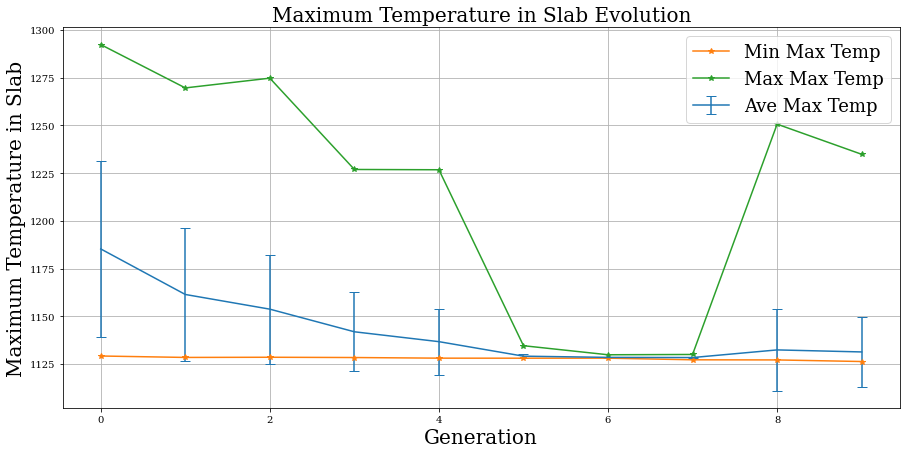
\includegraphics[width=\linewidth]{slab-obj-1-temp-evol.png}
        \caption{Minimum, average, and maximum evolution of $T_{max}$ in 
        AHTR plank.}
        \label{fig:slab-obj-1-temp-evol} 
    \end{subfigure}
    \begin{subfigure}{\textwidth}
        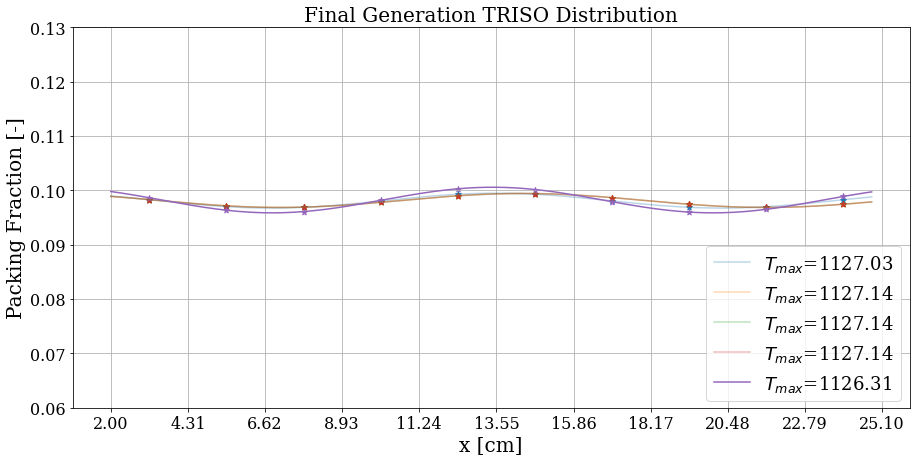
\includegraphics[width=\linewidth]{slab-obj-1-temp-final.png}
        \caption{TRISO particle distribution for the 5 individuals with the 
        lowest $T_{max}$ in AHTR plank at generation 9.}
        \label{fig:slab-obj-1-temp-final} 
    \end{subfigure}
    \caption{ROLLO single-objective optimization to minimize $T_{max}$ 
    in the plank. Input parameters varied: TRISO particle distribution.}
    \label{fig:slab-obj-1-temp}
\end{figure}
The minimum and average plank's $T_{max}$ converged to approximately 
1125 K. 
In Figure \ref{fig:slab-obj-1-temp-final}, a mostly flat TRISO 
particle distribution minimizes $T_{max}$ in the plank, the TRISO particle distribution 
has two small dips at the one-third and two-third points in the slab (6.62cm and 20.48cm). 
A fully flat TRISO particle distribution results in a higher $T_{max}$.
Figure \ref{fig:slab-obj-1-temp-distr} compares the Moltres-generated centerline 
temperature distribution for the plank with mostly flat (Figure 
\ref{fig:slab-obj-1-temp-final}) and flat TRISO particle distributions for the same 
total packing fraction.
\begin{figure}[]
    \centering
    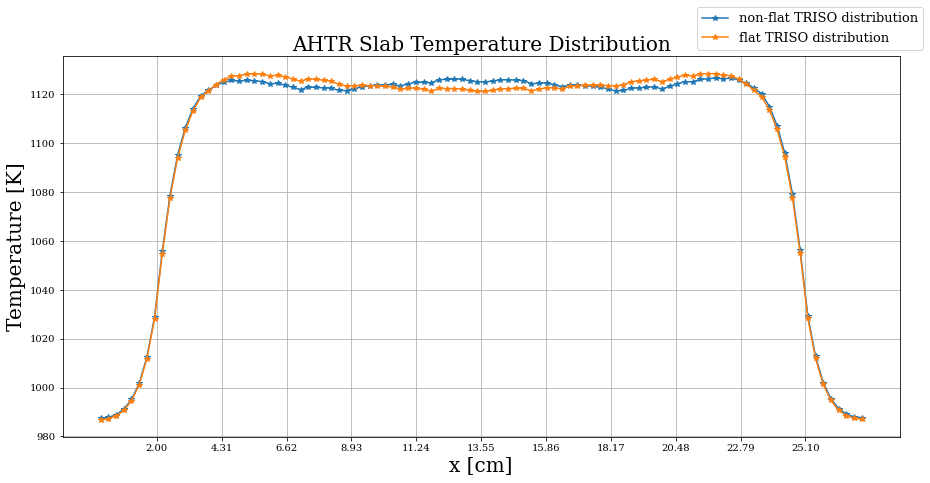
\includegraphics[width=\linewidth]{slab-obj-1-temp-distr.png}
    \caption{Comparison of Moltres-generated AHTR Plank Temperature Distribution for non-flat and flat
    TRISO distribution. Both models have a total packing fraction of 0.0979.}
    \label{fig:slab-obj-1-temp-distr}
\end{figure}
The AHTR plank with a flat TRISO particle distribution has higher plank temperatures 
on the left and right sides near the moderator. 
To combat this temperature peak, ROLLO found a TRISO particle distribution that 
has a slight dip near the moderator regions, resulting in a lower $T_{max}$.

\subsubsection{Simulation 1f: Variation of FliBe Channel Shape}

\subsection{Objective: Minimize Fuel-Normalized Power Peaking Factor}

\subsubsection{Simulation 1d: Variation of $\rho_{TRISO}(\vec{r})$}
Table \ref{tab:simulation1d} shows simulation 1d's optimization problem parameters. 
\begin{table}[H]
    \centering
    \onehalfspacing
    \caption{Simulation 1d Optimization Problem Parameters}
	\label{tab:simulation1d}
    \footnotesize
    \begin{tabular}{l|p{3cm}}
    \hline 
    \multicolumn{2}{c}{\textbf{Single Objective: Simulation 1d}} \\
    \hline 
    \textbf{Objectives} & Minimize $T_{max}$ \\
    \hline 
    \textbf{Input Parameter variations} & $0<a<2$ \\
    & $0<b<\frac{\pi}{2}$ \\
    & $0<c<2\pi$ \\
    \hline
    \textbf{Constraints} & $k_{eff} > 1.0$\\ 
    \hline 
    \textbf{Genetic Algorithm Parameters} & Population size: 60 \\
    & Generations: 10 \\
    \hline
    \end{tabular}
\end{table}
Figure \ref{fig:slab-obj-1-ppf-evol} shows the slab's normalized power peaking 
factor evolution and Figure \ref{fig:slab-obj-1-ppf-final} shows the five TRISO particle 
distributions in the final generation with the normalized power peaking factor.
\begin{figure}[]
    \centering
    \begin{subfigure}{\textwidth}
        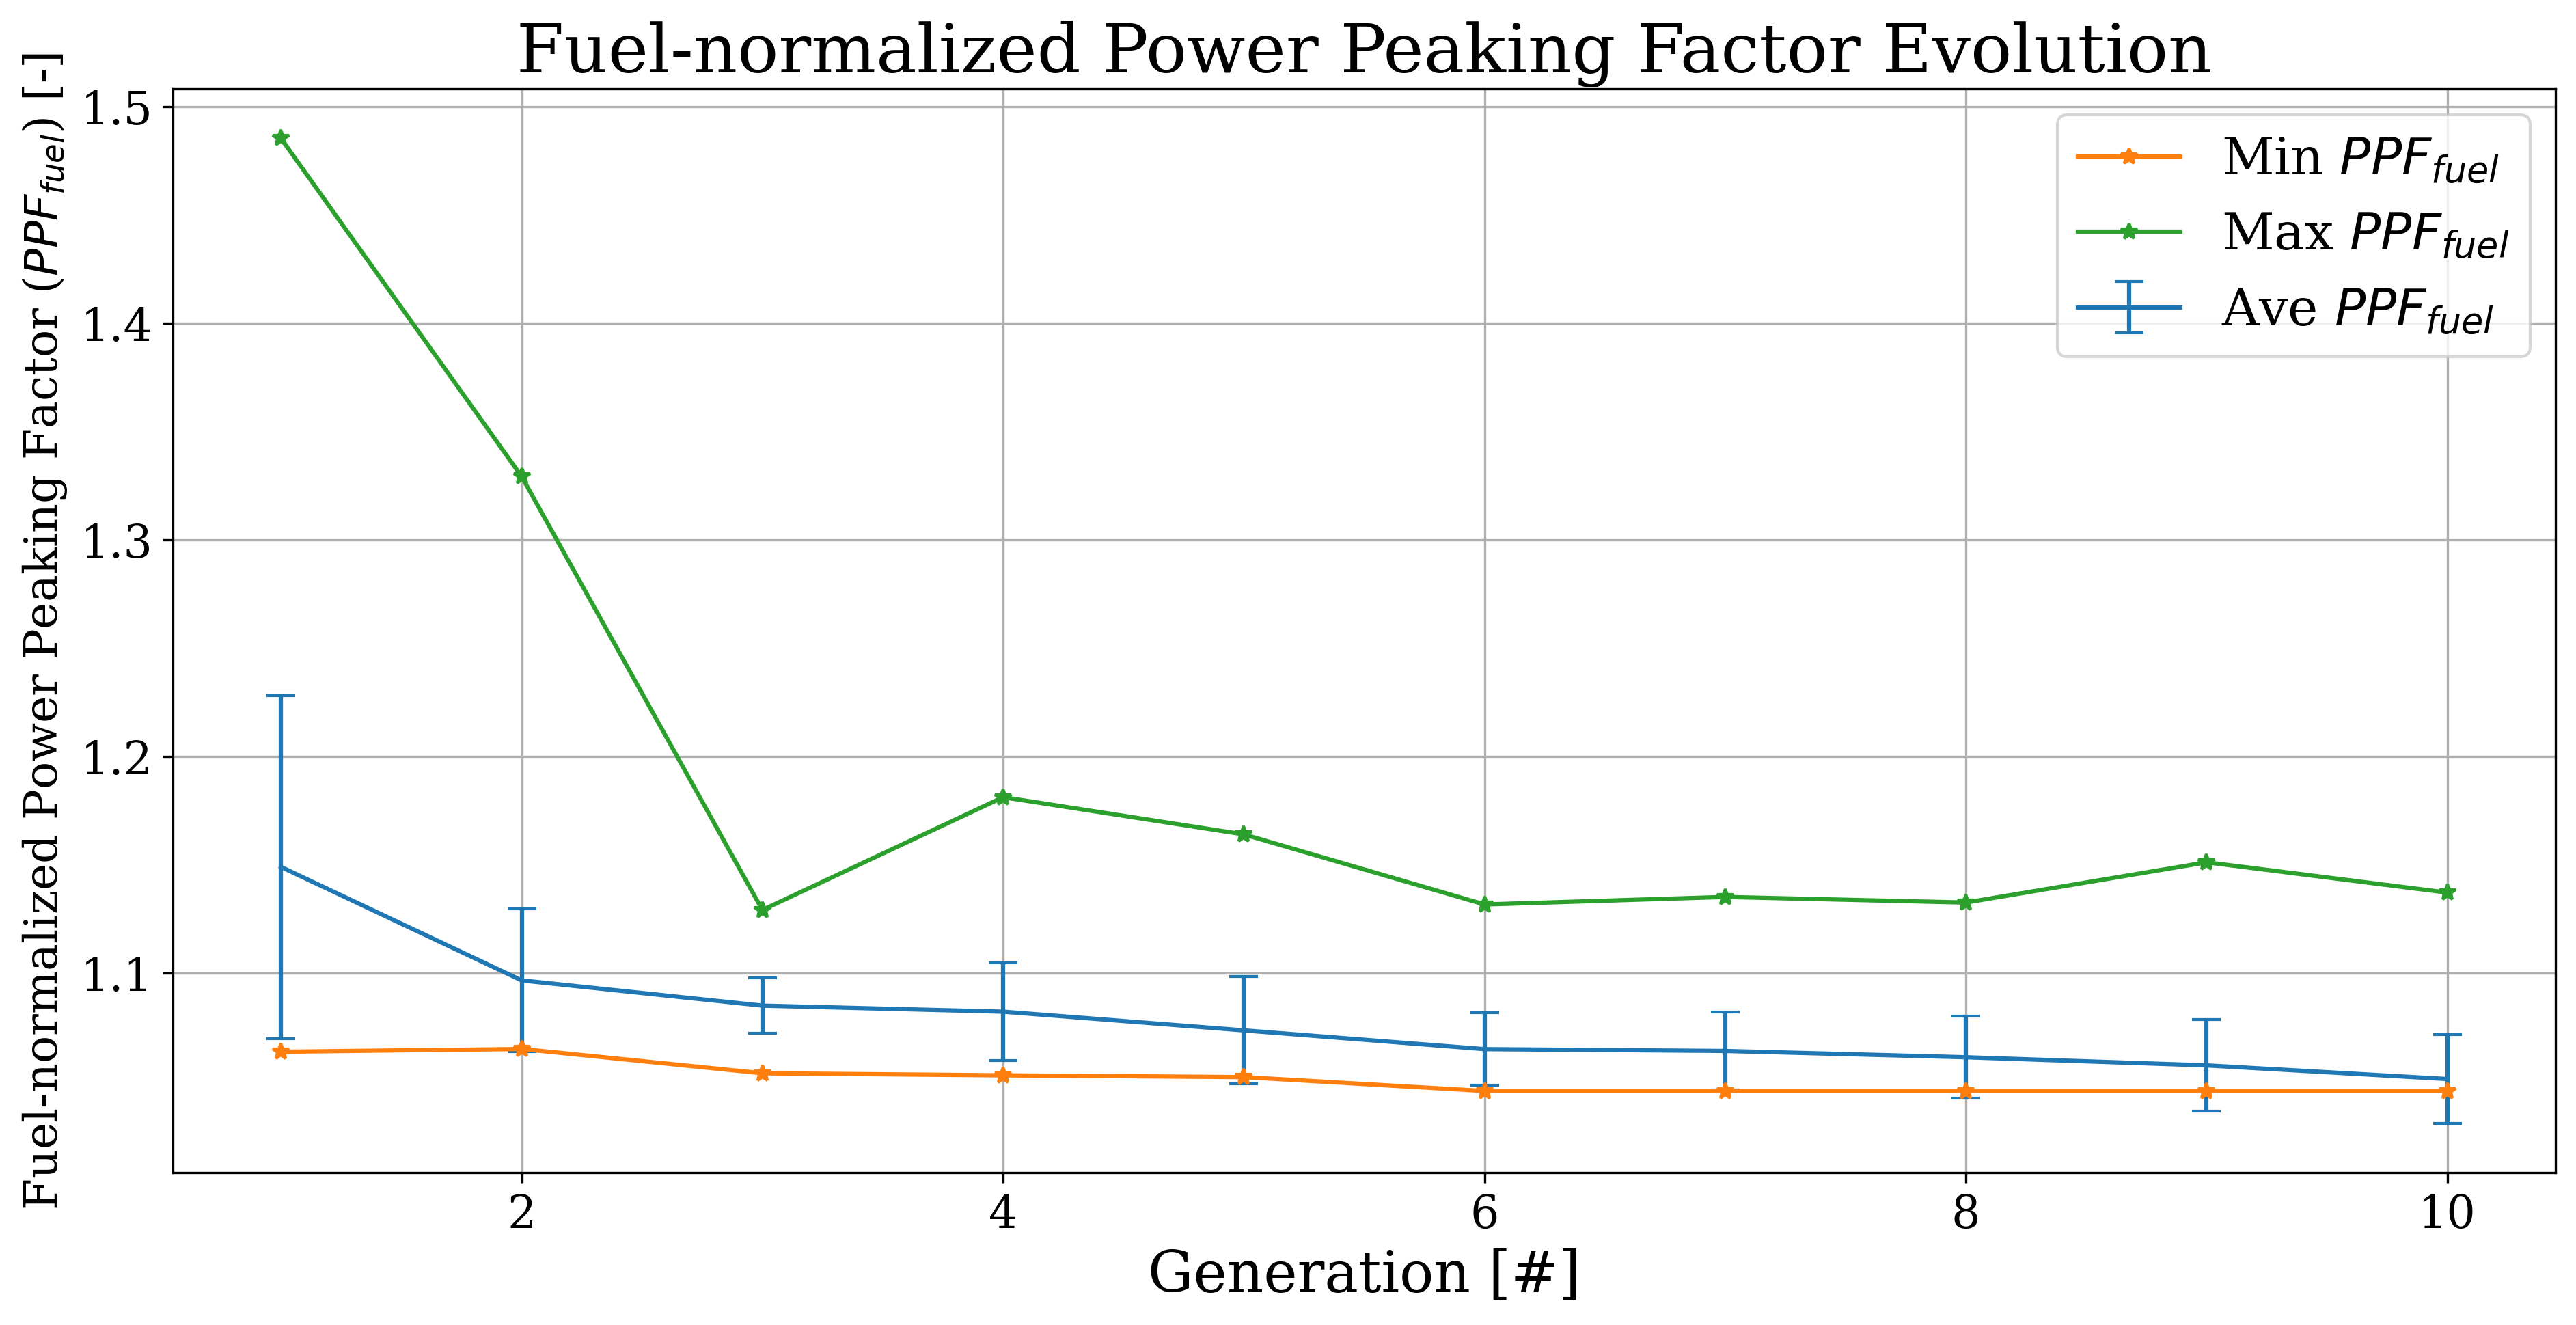
\includegraphics[width=\linewidth]{slab-obj-1-ppf-evol.png}
        \caption{Minimum, average, and maximum evolution of normalized power 
        peaking factor in AHTR slab.}
        \label{fig:slab-obj-1-ppf-evol} 
    \end{subfigure}
    \begin{subfigure}{\textwidth}
        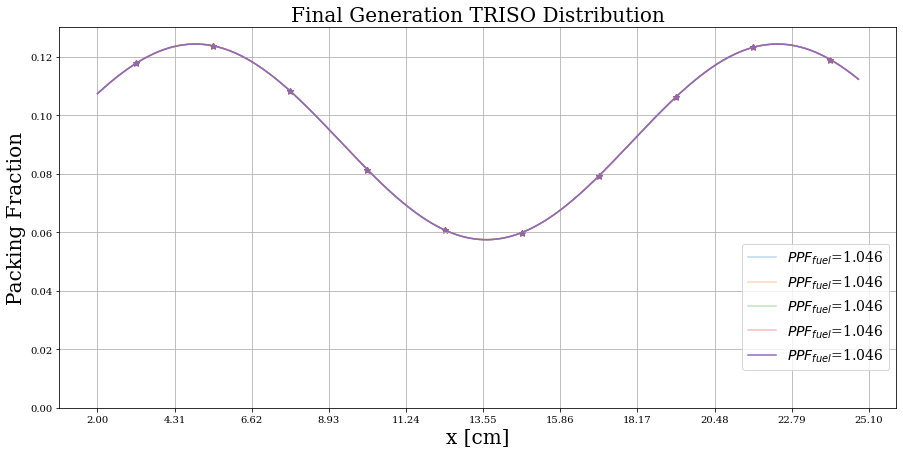
\includegraphics[width=\linewidth]{slab-obj-1-ppf-final.png}
        \caption{TRISO particle distribution for the 5 individuals with the 
        lowest normalized power peaking factor in AHTR slab at generation 9.}
        \label{fig:slab-obj-1-ppf-final} 
    \end{subfigure}
    \caption{ROLLO single-objective optimization to minimize normalized power 
    peaking factor in the slab. Input parameters varied: TRISO particle distribution.}
    \label{fig:slab-obj-1-ppf}
\end{figure}
In Figure \ref{fig:slab-obj-1-ppf-final}, the TRISO distribution that best minimizes 
PPF peaks near the edges of the fuel region of the plank, and has a minimum point in 
center of the plank.
This distribution is attributed to the self-shielding effects. 
The edges of the fuel region have higher flux as they are closer to the graphite 
moderator, whereas the plank's center has a lower flux due to self shielding. 
Thus, to minimize PPF, \gls{ROLLO} found a plank TRISO distribution that has higher 
packing fraction at the edges, and a lower packing fraction in the center. 

\subsubsection{Simulation 1g: Variation of FliBe Channel Shape}

\section{AHTR Plank: Two-Objective Optimization Results}

